\section{Dataset}
\label{sec:real_world_dataset}
For the real-world validation, the focus will be on testing the model on the \textbf{multi-variation} \textit{Pick-Place} tasks, focusing on a smaller set of variations compared to the complete 16 variations described in Section \ref{sec:cod_dataset}.

\begin{figure}[t]
    \centering
    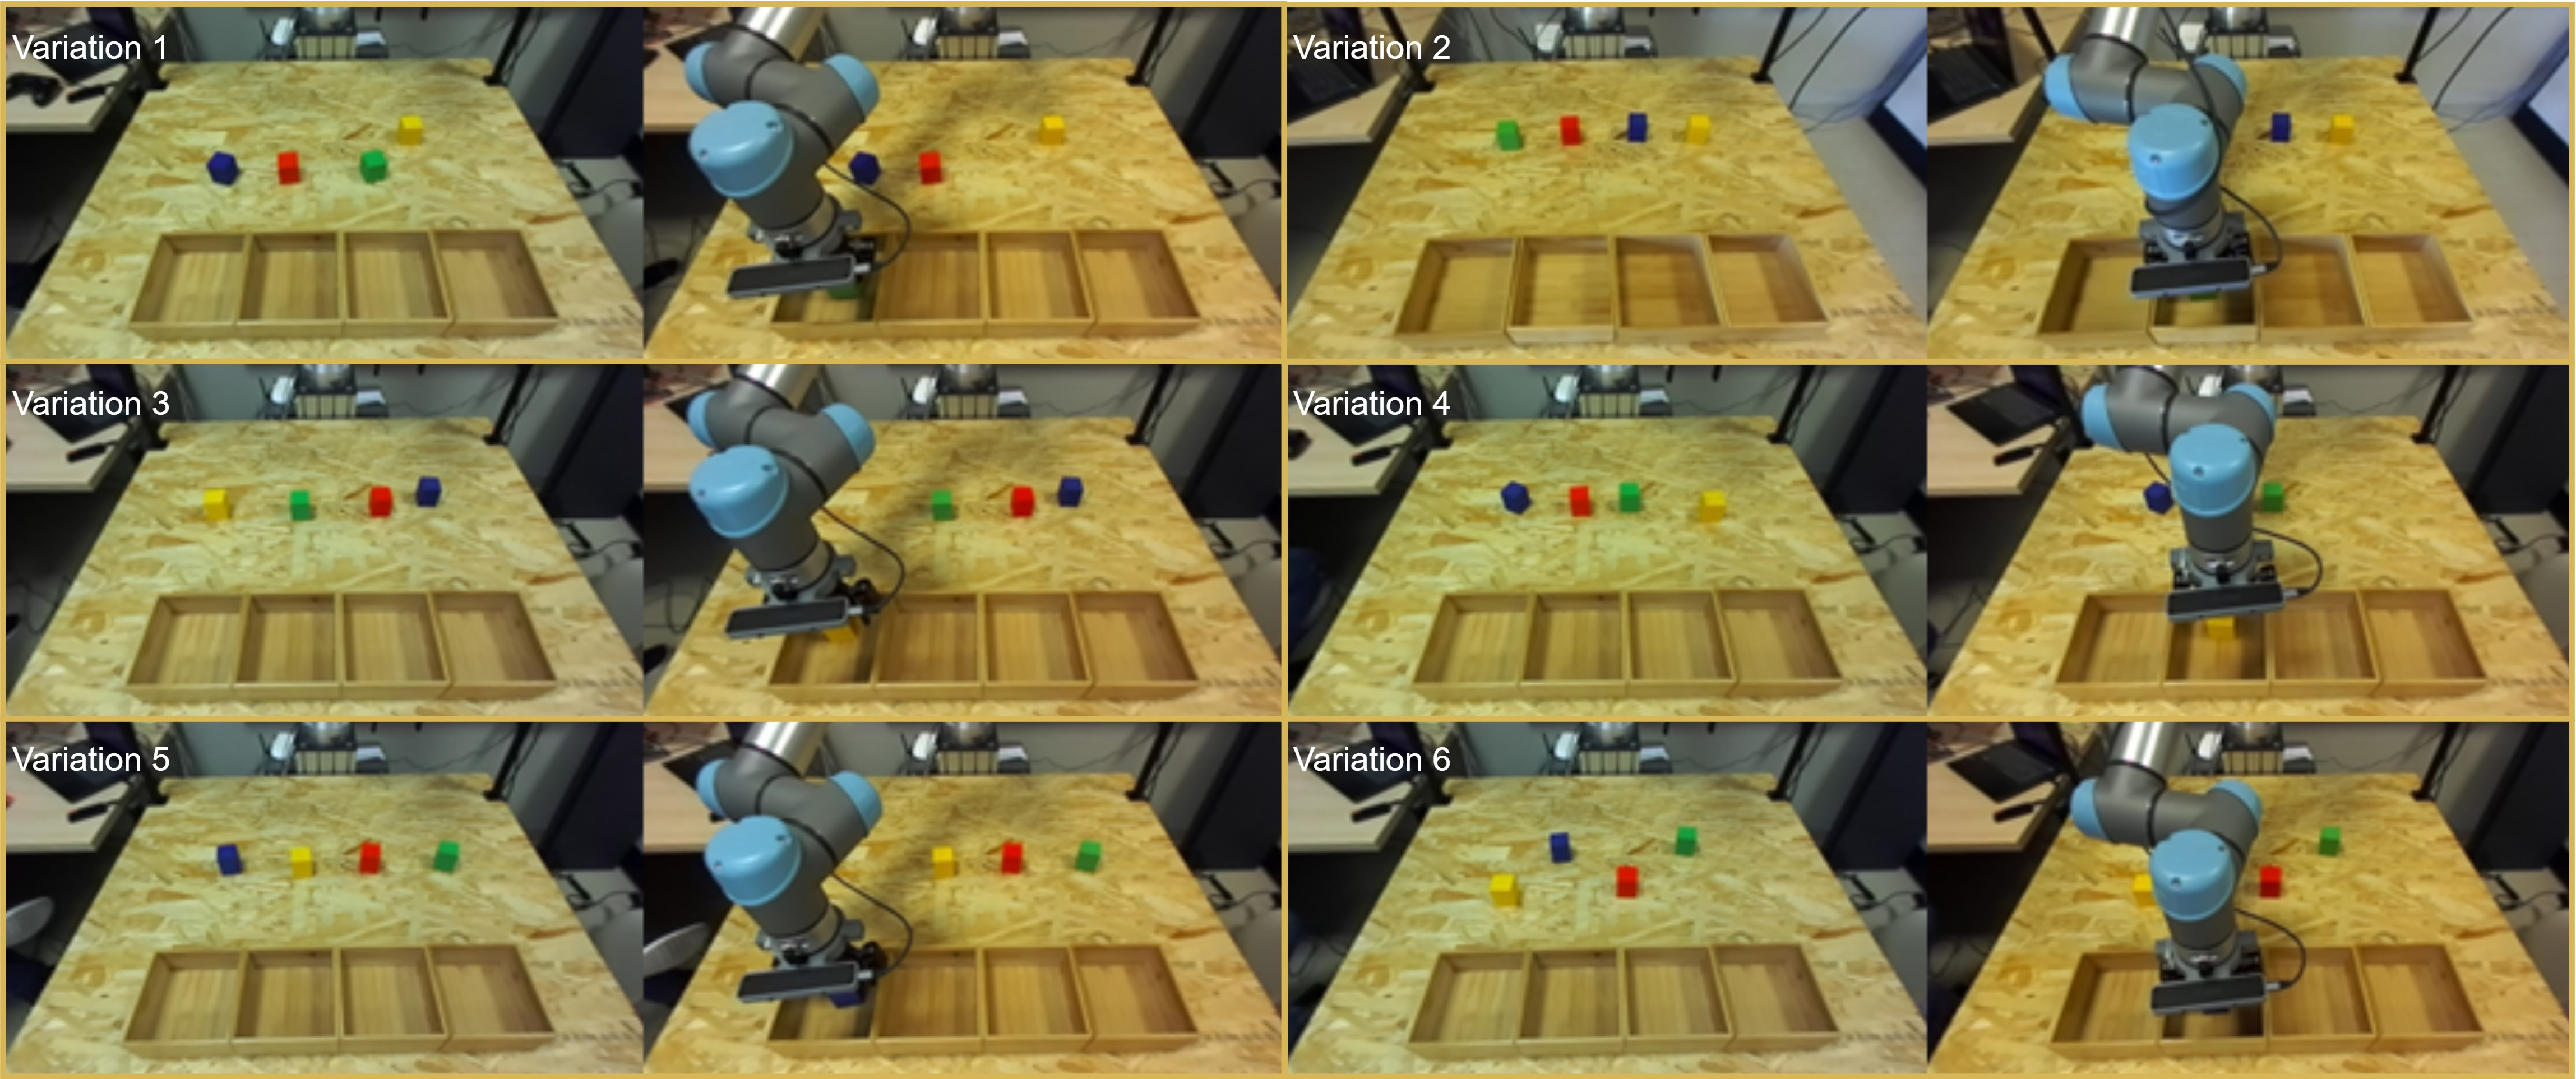
\includegraphics[width=1.0\textwidth]{figures/images/ch5/real_world_dataset.jpg}
    \caption{Set of variations used in the real-world robot evaluation. For each variation, the first and last frames are provided}
    \label{fig:real_world_dataset}
\end{figure}


Figure \ref{fig:real_world_dataset} represents the 6 variations used in the real-world validation. As can be noted, these are essentially the first six variations of the Pick-Place Task used in the simulation environment.

A preliminary dataset composed of \textbf{40 trajectories} for each variation has been collected by teleoperating the robot with a console controller. Regarding the object placement, the same algorithm described in Section \ref{sec:ocpl_dataset} was applied. This means that the set of 4 bins ($15 \times 15 \times 7$ cm) was fixed in position, while the 4 boxes ($4 \times 4 \times 6$ cm) could vary in their position within a region of $60$ cm in length and $15$ cm in height. 

In this large placement region, a specific protocol was implemented for collecting the trajectories. The protocol is related to how the objects are placed in the picking region. The different placements of the target object are reported in Figure \ref{}.
\smalltodo{add figure}
% \smalltodo{add figure}
Trajectories are collected through teleoperation the robot is controlled in its operational space, with the controller that sends continous velocity commands on a specific axis, this velocity command is defined by the value read by the controller's potentiometers.
During teleoperation different informatin are recorded:
\begin{itemize}
    \item \textit{Images} from the front, laterals and gripper cameras, both RGB and Depth images are recorded.
    \item \textit{Proprioceptive information} like joints positions and velocities.
    \item \textit{Trajectory state}, which is manually changed by the human operators based on the task state. The phases are:
        \begin{enumerate}
            \item \textit{Start}, this phase starts at the beginning of the trajectory till the robot gripper is perpendicular to the target object.
            \item \textit{Approaching}, this phase starts when the robot approaches the target object with its discending movement.
            \item \textit{Picking}, this phase is characterized by the gripper that is ready to be closed to pick the object, and contains the closing command.
            \item \textit{Moving}, this phase starts after the robot picks the object and lift it from the table, this phase ends when the gripper is perpendicular to the target bin.
            \item \textit{Placing}, this phase starts when the robot is ready to place the object, starting the discending phase towards the target bin, this phase also contains the opening command.
        \end{enumerate}
    \item \textit{Objects bounding boxes}, which are are generated automatically, requiring minimal input from human operators. At the start of the trajectory, the operator needs to specify the position of each object in the scene, including both boxes and bins. This is done by displaying the first frontal frame of the trajectory and clicking on the objects with the cursor. The positions, initially defined in discrete pixel-space, are then converted into continuous world-space through a series of transformations, using the camera's intrinsic and extrinsic parameters. The extrinsic parameters are obtained via a calibration procedure that uses ARUCO markers.
\end{itemize}
The overall space coverage of the real-world dataset is shown in Figure \ref{}. As can be observed, the coverage is more limited and considerably noisier compared to the simulated dataset, even when restricted to the same variations. This is due to the collection of fewer trajectories and the use of teleoperation without any hand-written control rules, which typically generate smoother and more deterministic robot behaviors. These limitations introduce additional challenges in learning a robust control policy, especially for generalizing to different placements of the target object. This issue will be addressed in this thesis by initially training the policy in the simulation environment, where a complete dataset is available, and then fine-tuning it on the noisy real-world dataset.
\smalltodo{add figure}